%===============================================================================
\section{Luminosity function estimation: Framework}
\label{sec:lum_func}

The CUDAHM distribution contains some example code implementing basic hierarchical models, such as the normal-normal model, and a realistically complicated astrophysical example handling regression with classical measurement error, with nonlinear models (the interstellar dust problem described above).

As a somewhat more complicated application of CUDAHM, we here consider luminosity function estimation, a parametric conditional density estimation problem arising across many areas of astronomy.
We highlight this example, both because of its ubiquity across astronomy, and to illustrate the generality of CUDAHM.
We describe luminosity function estimation for a model including not only measurement error, but also \emph{selection effects}.
The selection effects make the joint distribution structure more complicated than the conditional density estimation DAG shown in Fig.~\ref{fig:DAGs}; in particular, there are two plates (corresponding to detected and undetected objects).
However, the likelihood function can be manipulated to have a conditional dependence structure similar to that of a single-plate DAG, allowing straightforward implementation of the model using CUDAHM.

%-------------------------------------------------------------------------------
\subsection{Astronomical background}
\label{sec:LF-astro}

%\enote{Introductory content here was moved from Janos's intro.}

The fundamental observables for localized astronomical sources include position (both direction on the celestial sphere, and distance, $r$, in some chosen coordinate system), and apparent brightness, quantified in terms of flux, $F$ (energy or photon number per unit time per unit area normal to the line of sight).
Astronomers use these observables to study demographic properties of many classes of sources, including stars and galaxies of various types, minor planets (such as asteroids), and explosive transients (gamma-ray bursts, supernovae).
For concreteness, here we focus on observations of nearby galaxies, for which distance may be measured by using spectroscopy to find the \emph{redshift}, $z$, of spectral lines (i.e., their fractional shift in wavelength from laboratory values).
Due to the cosmological expansion, for relatively nearby galaxies outside the local group, distance is proportional to redshift to a good approximation, with
\begin{equation}
r = \frac{cz}{H_0},
\label{eq:H0}
\end{equation}
where $c$ denotes the speed of light, and $H_0$ is Hubble's constant, measuring the current expansion rate of the universe, with $H_0 \approx 70$~km~s$^{-1}$~Mpc$^{-1}$ (with Mpc denoting megaparsecs).
$H_0$ is measured with a precision of several percent, and spectroscopic redshifts for nearby galaxies can be measured to sub-percent precision.
For simplicity, here we consider distances to be precisely measured, via spectroscopic redshifts.
Often, astronomers use redshift directly as a proxy for distance.

A fundamental intrinsic characteristic of a source is its \emph{luminosity} (emitted power), $L$, a measure of its intrinsic (vs.\ apparent) brightness (with units of energy per unit time).
For nearby galaxies (i.e., for distances where space is very nearly Euclidean), the inverse-square law relates $L$ to the observables $F$ and $r$:
\begin{equation}
F=\frac{L}{4\pi r^2}.
\label{eq:inv-sqr}
\end{equation}
The \emph{luminosity function}, $\lfunc(L, r)$, describes the distribution of luminosities for a population at a specified distance (or redshift).
It is typically defined as the intensity function for a point process, i.e., as specifying the expected number of galaxies per unit volume at distance $r$, per unit luminosity interval.
If we denote the spatial number density of galaxies at distance $r$ by $n(r)$, then $n(r) = \int dL\, \lfunc(L, r)$.
The \emph{luminosity PDF} for galaxies at distance $r$ is then
\begin{equation}
\lpdf(L,r) = \frac{\lfunc(L, r)}{n(r)}.
\label{eq:lpdf}
\end{equation}
Note that $\lfunc(L,r)$ and $\lpdf(L,r)$ specify \emph{conditional} distributions, i.e., distributions for $L$ at a given $r$.%
\footnote{Authors vary on the definition of the luminosity function, many defining it as done here, and others using ``luminosity function'' to denote what we here call the luminosity PDF.}
Using (\ref{eq:inv-sqr}), the \emph{flux PDF} for galaxies at distance $r$, denoted $\rho(F,r)$, can be found by a change of variables from $L$ to $F$, giving
\begin{equation}\label{eq:fluxPDF}
\rho(F,r) = 4\pi r^2 f(4\pi r^2 F, r).
\end{equation}

The galaxy luminosity function carries valuable information about the formation and evolution of galaxies, therefore it is an important target of inquiry in astronomy (see \citealt{BST88-LumFuncReview} and \citealt{J11-LumFuncReview} for reviews).
\citealt{J11-LumFuncReview} provides a review of methods developed by astronomers for estimation of galaxy luminosity functions.
CUDAHM can address parametric luminosity function inference; this section provides an example as a demonstration of CUDAHM's capability and flexibility.
In the next subsection, we describe a useful parametric family of luminosity functions.
Then we present a hierarchical Bayesian framework for modeling astronomical survey data using thinned latent marked point process models, developing it specifically for luminosity function inference.
The next section presents a simulation study demonstrating CUDAHM luminosity function inference for simulated populations with sizes up to $10^6$.

% For simplicity we here focus on a homogeneous population, so that $n(r)$ is considered fixed (constant with respect to volume measure).
% The following development is straightforward to generalize to account for models with distance dependence in the luminosity function.

%-------------------------------------------------------------------------------
\subsection{Parametric luminosity function models}
\label{sec:lfmodels}

For most cosmic populations, including galaxies, the luminosity function falls very steeply with increasing luminosity.
The canonical starting point for parametric modeling of luminosity distributions is the \emph{Schecter function},
\begin{equation}
\lfunc(L;\theta) =
  \frac{A}{L_*} \left(\frac{L}{L_*}\right)^{\beta} e^{-L/L_*},
\label{eq:schecter}
\end{equation}
where the parameters $\theta = (L_*,\beta, A)$ comprise a luminosity scale, $L_*$, a power law index, $\beta$, and an amplitude, $A$.%
\footnote{There are varying conventions for parameterizing the amplitude of the Schecter function.
In this parameterization, $A$ has units of space density.
In similar parameterizations, $A$ is often denoted $\lfunc_*$, although it neither has the units of $\lfunc$, nor is it equal to $\lfunc(L_*)$, as the symbol might misleadingly suggest.}
The form of the Schecter function would seem to imply a luminosity distribution that is a gamma distribution (with shape parameter $\alpha = \beta - 1$).
However, the observed samples of many populations follow Eq.~\ref{eq:schecter} with $\beta$ in the interval $(-2,-1)$, in which case the integral of $\lfunc(L;\theta)$ over $L$ is infinite, and the luminosity distribution is formally improper (with $\alpha$ outside of the allowed range for the gamma distribution).
Low-luminosity sources are unobservable (due to noise and background, discussed below), so in practice the \emph{observable} luminosity function is truncated at low luminosities, and the impropriety is often ignored.
But the actual luminosity function must rise less quickly with decreasing $L$ (corresponding to $\beta$ becoming larger than $-1$) or be cut off at low luminosities (corresponding to there being a minimum galaxy size).

%\enote{Perhaps move some of the following details to an appendix?}

For some populations, an increase in the power law index (i.e., flattening of the logarithmic slope) is in fact observed at low luminosities.
This has been observed for quasars (galaxies with a large, actively accreting central black hole; see \citealt{M+13-QuasarLumFunc}).
Similarly, the stellar initial mass function (related to the stellar luminosity function, and fit with similar models) has a low-mass (low-luminosity) index that flattens by $\approx 1$ (\citealt{K07-IMF-BPL}).
Motivated by such observations, and to keep the luminosity distribution proper, we here adopt a ``break-by-one'' (BB1) generalization of the Schecter function, with $\lfunc \propto L^{\beta+1}$ at low luminosities, and thus integrable for $\beta > -2$.
Specifically, the BB1 model has a luminosity distribution with three parameters: a mid-luminosity power law index, $\beta$, and two parameters defining the mid-luminosity range, $(l, u)$, with $l < u$ and  $u$ playing the role of $L_*$ in the Schecter function, and the power law index smoothly breaking to $\beta+1$ as $L$ decreases below $l$.
The BB1 luminosity PDF has following functional form:
\begin{equation}
\label{eq:lumPDF} 
\lpdf(L ; \theta) = 
  \frac{C(\beta,u,l)}{u}\left(1-e^{-L/l}\right) \left(\frac{L}{u}\right)^{\beta} e^{-L/u},
\end{equation}
where the normalization constant $C(\theta)$ is
\begin{equation}
\label{eq:normLumPDF} 
C(\beta,u,l) =
  \begin{cases} \dfrac{1}{\Gamma(\beta+1)\cdot\left(1-\frac{1}{\left(1+\frac{u}{l}\right)^{\beta+1}}\right)} 
    & \quad \text{if } \beta > -2\text{ and }\beta \ne -1; \\
 \dfrac{1}{\log\left(1+\frac{u}{l}\right)} & \quad \text{if } \beta=-1.
  \end{cases}
\end{equation} 
Note that as $l\rightarrow 0$, the BB1 distribution becomes a gamma distribution (if $\beta > -1$).
%Also, in our computational implementation, the condition $\beta=-1$ of the first case is $-1.001<\beta<-0.999$.
We designed the BB1 distribution to have smooth power law break behavior at low $L$, yet also have an analytical normalization constant;
it is proper for $\beta > -2$.
It can also be sampled from using a straightforward modification of a widely-used algorithm for sampling from the gamma distribution (\citealt{ahrens_computer_1974}).
These properties make it useful for simulation experiments.

We define a BB1 luminosity function by multiplying the BB1 luminosity distribution by the galaxy spatial number density, which is simply a constant, $n$, for a homogeneous population.
Fig.~\ref{fig:lumfunc} shows an example BB1 luminosity function, with $\beta = 1.5$, and $(l,u) = (5\times 10^{10}, 5\times 10^{12})$ in dimensionless units; it is plotted both with $\log$-linear axes, and with $\log$-$\log$ axes, where the varying power law behavior is evident.
The local power law index corresponds to the slope, $G(L)$, in $\log$-$\log$ space, defined by
\begin{equation}
	G(L) \equiv \frac{\dd\log{\lpdf}}{\dd\log{L}} = \frac{L}{\lpdf} \frac{\dd \lpdf}{\dd L} = g(L) + \beta - \frac{L}{u},
\end{equation}
with
\begin{equation}
	g(L) = \frac{L}{l}\cdot\frac{1}{e^{L/l} - 1}.
\end{equation}
Evidently, $g(L) \rightarrow 0$ for $L \gg l$ and $g(L) \rightarrow 1$ for $L \ll l$.
Thus the logarithmic slope, $G(L)$, corresponds to an exponential cutoff at large $L$, and at small $L$, a slope of $\beta + 1$.
When $u\gg l$, so there is a range where $L\gg l$ but $L\ll u$, the logarithmic slope is $\approx \beta$ in that range.

\begin{figure}
	\begin{subfigure}[c]{0.45\textwidth}
		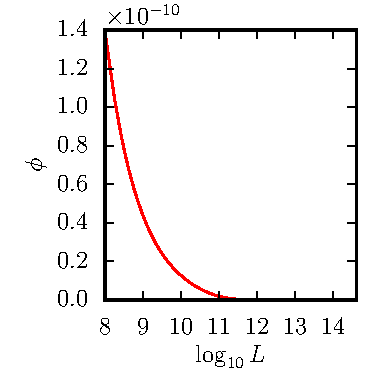
\includegraphics{fig/lumfunc_loglin}
		\caption{}
	\end{subfigure}
	\begin{subfigure}[c]{0.45\textwidth}
		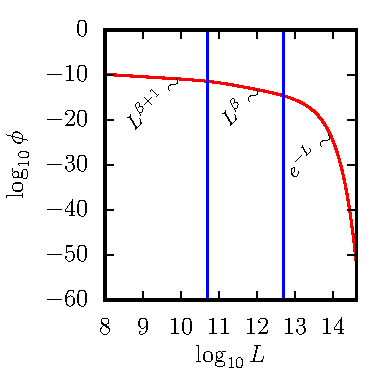
\includegraphics{fig/lumfunc_loglog}
		\caption{}
	\end{subfigure}
	\caption{Example BB1 truncated broken power law PDF, on a log-linear scale (a) and on log-log scale (b), with parameters $(u,l) = (5\times 10^{10}, 5\times 10^{12})$ in dimensionless units, and $\beta = -1.5$.
	In Panel~b the blue verticals show the lower limit $l$ and upper limit $u$ of the region where the power law slope is $\approx\beta$.}
	\label{fig:lumfunc}
\end{figure}

Finally, the BB1 cumulative distribution function is 
\begin{equation}
\label{eq:lumCDF} 
\lcdf(L ; \theta) = 
  C(\theta)
  \left[ \Gamma(\beta + 1) - \gamma\left(\beta + 1, L/u\right) - \frac{\Gamma(\beta + 1)-\gamma\left(\beta + 1, L\cdot\left(\frac{1}{u}+\frac{1}{l}\right)\right)}{\left(1 + \frac{u}{l}\right)^{\beta + 1}} \right],
\end{equation}
where $\Gamma(\cdot)$ and $\gamma(\cdot, \cdot)$ denote the gamma function and the upper incomplete gamma function, respectively.

%-------------------------------------------------------------------------------
\subsection{Modeling survey selection effects and measurement error}
\label{sec:slxn+err}

Astronomers estimate luminosity functions and other astronomical distributions using data compiled in \emph{survey catalogs}: tables of estimates (including uncertainties) of object properties, accompanied by a description of selection criteria for the survey that produced the catalog.
Catalogs are derived data products; they summarize information in more complex and voluminous raw datasets, such as large collections of images or time series.
The nature of astronomical catalog data makes their analysis differ in some respects from analyses of survey data familiar in the statistical survey sampling literature.

Flux measurements are affected by measurement error that is often dominated by Poisson fluctuations in the photon counting rate, including fluctuations from astrophysical and instrumental backgrounds.
The measurement error thus approximately scales with the square root of the flux, and is fractionally greater at low flux than at high flux.
At low fluxes, photons from the backgrounds can produce false source detections.
To prevent this, surveys adopt detection criteria to strongly mitigate against false detections.
A simple, representative criterion is to accept sources only if the estimated flux is $\nu$ times the flux uncertainty, with $\nu \approx 5$ so that the probability for false detection is low even for large catalogs (i.e., there is strong control of the family-wise error rate).

Detection criteria introduce \emph{selection effects} into catalogs.
Most obviously, faint sources (low luminosity sources, or distant high luminosity sources) are excluded; the observable luminosity function is a thinned version of the actual luminosity function.
In addition, \emph{measurement error} more subtly but significantly distorts the shape of the observable distribution, a phenomenon well known in the density deconvolution literature, and also recognized in the astronomical literature, where it is sometimes called \emph{Eddington bias}, in reference to early discussions of the distortion by Eddington and Jeffreys (REFS).
They noted that an object with a measured flux of $\hat F$ is more likely to be an object with a true flux $F < \hat F$ than one with $F > \hat F$, even when measurement errors have a symmetric distribution, because dim sources are more numerous than bright sources in most astronomical settings.
Selection effects can exacerbate the distortion in the vicinity of a flux threshold, with measurement error and the falling flux distribution conspiring to scatter more below-threshold sources into the observed sample than above-threshold sources out of it, a component of what astronomers call \emph{Malmquist bias} \citep{binney1998galactic} (although the term is used inconsistently).
Hierarchical modeling can automatically account for such thinning and distortion, in a manner that adapts to the shape of the luminosity function; this is a major motivation for its increasing popularity in astrostatistics.

We have developed a framework for modeling astronomical survey data using \emph{thinned latent marked point process models}.
Measurement error is handled in a hierarchical Bayesian manner, by introducing latent member property parameters, with catalog estimates understood as describing member likelihood functions for the properties.
We model the population distribution of the latent member properties using marked point processes.
We model selection effects through thinning of the latent point process.
This framework was originally developed for studying the luminosity function of gamma-ray bursts, powerful explosive transients thought to mark the birth of stellar-mass black holes (\citealt{LW95-GRBs-TLPP,LW98-GRBs-Iso}).
It was subsequently adapted to study the luminosity distribution (and through it, the size distribution) of trans-Neptunian objects, asteroid-like minor planets in the outer solar system (\citealt{L04-MsmtErr,P+08-TNOSizeDistn}).
We outline the framework here as it applies to luminosity function estimation and similar problems, in contexts where a marked Poisson point process is an appropriate model for the latent member properties.
\cite{kelly2008flexible} independently developed a similar approach for settings where a binomial point process may be appropriate, and applied it to estimating the number density of quasars as a function of redshift.

A somewhat subtle aspect of the problem is the tie between measurement error and selection effects.
In astronomical surveys, the raw data are searched to find candidate objects.
For candidates that pass detection criteria, the data are used to estimate source properties.
The same underlying data are used both for selection (detection) and measurement; these tasks are not independent, as is assumed in many statistical survey methods outside of astronomy.
Ignoring the dependence can corrupt inferences.

Object detection is typically implemented via a scanning procedure.
For example, for image data, a fixed aperture may be scanned over the image; a detection algorithm determines if an object is present, e.g., by comparing the estimated flux in the aperture to a threshold value (set by background and noise estimates), or by fitting an image model to the data in the aperture and comparing the fitted amplitude to a threshold.
For time series data, a window may be scanned over the time series, with an object detected if the estimated flux is above a threshold.
If an object is detected, its properties are estimated, e.g., by a likelihood or weighted least squares calculation, with estimation results summarized in the catalog.

Fig.~\ref{fig:ScanMark} illustrates the framework and its relationship to catalog construction.
We split the object property parameter space into scan and mark components.
The scan component corresponds to the dimensions over which the detection scan operates; 
%(e.g., two-dimensional position for image data, or arrival time for time series data).
the mark component corresponds to the remaining dimensions.
For our galaxy luminosity function example, the scan component is the two-dimensional position of the galaxy image on the detector (corresponding to its direction on the sky), and the mark component is the galaxy luminosity and distance, or equivalently, flux and distance (in a more complex case, the mark component might include color and morphological parameters).
In the figure, the dots (red) indicate the true properties of seven galaxies; the blue contours depict likelihood functions for the properties, based on noisy image data.
The gray region at the bottom is bounded above by the position-dependent detection threshold; an object is detected only if its best-fit (maximum likelihood) flux is above the threshold.
Here two of the seven galaxies are not detected.

\begin{figure}
\begin{center}
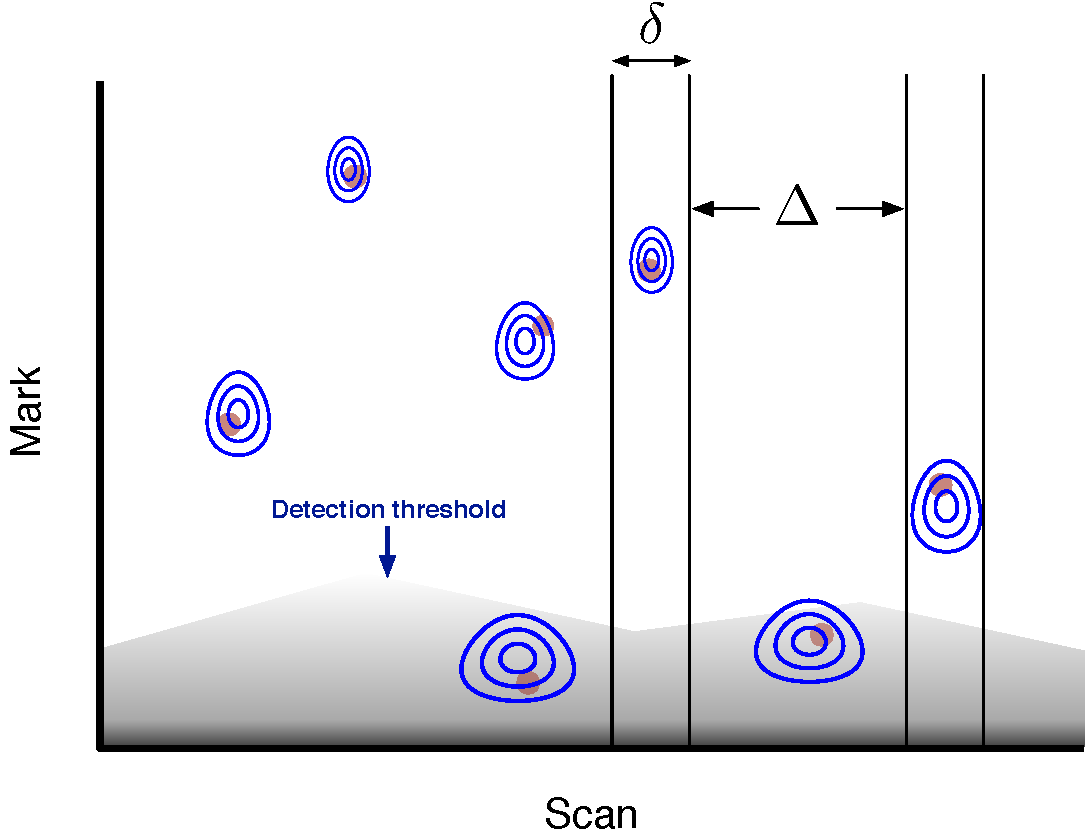
\includegraphics[width=.8\textwidth]{fig/ScanMarkPtProcess-Thin+Err}
\end{center}
\caption{Depiction of thinned latent marked point process model for catalog data produced by an astronomical survey.
Object properties are split into a scanned subset and a mark subset.
Dots (red) show latent (true) values for an object's properties.
Contours (blue) depict member likelihood functions from analysis of the raw survey data; catalogs provide summaries of these for detected objects.
Gray region at bottom depicts the non-detection region; candidates with estimated mark values below a varying threshold are rejected.
$\delta$ and $\Delta$ denote sizes of detection and nondetection intervals.}
\label{fig:ScanMark}
\end{figure}

We model the properties using a (latent) marked Poisson point process, i.e., a Poisson point process for the scanned parameters, and a probability density function for the mark parameters.
For concreteness, we focus on the luminosity function example, taking the scan parameter to be object position, $x$ (a 2-vector), and the mark parameters to be flux and distance, $(F, r)$.
We suppose that the spatial density of galaxies is approximately constant over the region probed by the survey.
There is thus a constant Poisson intensity parameter, $\lambda$, describing the distribution of galaxies in $x$.
We assume a BB1 luminosity PDF, independent of distance (of course, the flux PDF will depend on distance, thanks to the inverse square law).
The flux and distance mark PDF is thus a product of PDFs, $h(r)\rho(F,r)$.
For $\rho(F,r)$ we adopt the BB1 luminosity PDF form of (\ref{eq:lumPDF}), with parameters $\rhopar = (\beta,u,l)$, related to $\rho(F,r)$ via (\ref{eq:fluxPDF}); we write the flux PDF as $\rho(F,r; \rhopar)$ when we want to display the parameter dependence.
For the PDF for galaxy distance, $h(r)$, the assumption of homogeneity implies
\begin{equation}\label{eq:distPDF}
h(r) = 
\begin{cases} 
    \dfrac{3r^{2}}{r_u^{3}} & \quad \text{if } 0\leq r\leq r_u,\\
    0 & \quad \text{otherwise},
\end{cases} 
\end{equation}
where $r_u$ is an upper limit on distance chosen to be beyond the surveyed volume.%
\footnote{That is, chosen so that the most luminous galaxies of interest (i.e, with $L$ of order $u$ in the BB1 model) have fluxes comfortably below the lowest flux threshold.
In deep surveys (reaching to very dim fluxes), cosmological considerations, including the finite age of the universe and the non-Euclidean geometry of spacetime, ameliorate the growth of $h(r)$ with $r$.}
The population model thus has parameters $\ppar = (\lambda,\rhopar)$.

We consider a case where we have precise distance measurements for the galaxies (e.g., from high-resolution spectroscopic data providing precise redshifts).
We assume independent errors in the position and flux measurements, so the catalog contains descriptions of separate member likelihood functions for flux and position, denoted $\ell_i(F)$ and $m_i(x)$ for galaxy $i$, with $i=1$ to $N$.
Formally, denoting the image data for detected galaxy $i$ by $D_i$, we are writing
\begin{equation}\label{eq:xFr-like}
p(D_i|x,F,r) = \ell_i(F)\, m_i(x)\, \delta(r - r_i),
\end{equation}
where the Dirac delta function factor represents the precise measurement of distance.
We must also describe the survey's selection effects.
These are determined by the detection threshold as a function of the scan location.
At each scanned location, $x$, the threshold determines the set, $\dtxns_x$, of possible data (i.e., images) that would be deemed detections.
For example, if the detection criterion is that the MLE flux estimate, $\hat F(D)$ for data $D$, must exceed a threshold $\Fth(x)$, then $\dtxns_x = \{D : \hat{F}(D) > \Fth(x)\}$.
Reporting $\dtxns_x$, or equivalently $\Fth(x)$, then describes the selection effects.
But we will see below that a simpler summary of the detection criteria will suffice.


We now compute the likelihood function for the parameters, based on catalog data describing member likelihood functions and the selection effects.
The construction we use is illustrated in Fig.~\ref{fig:ScanMark}.
We partition the scan space into $N$ detection intervals, $\delta_i$, containing a single detected object, and $M$ nondetection intervals, $\Delta_j$, in which no candidate object passed the detection criterion.%
\footnote{We are presuming that galaxy images are well-separated, i.e., we do not treat here the \emph{crowded field} case, where the images of distinct objects may strongly overlap.}
The likelihood function is the product of the (conditionally independent) probabilities for these intervals.

We first consider the probability for no detection in one of the $\Delta_j$ intervals.
We break it up into subintervals of size $\delta x$, small enough that the detection threshold is approximately constant over the interval.
The probability for seeing no detections in $\delta x$ is the sum of the probabilities for the following events (conditioned on the population parameters, $(\lambda,\rhopar)$):
\begin{itemize}
\item No objects have $x$ in the interval.
\item One object has $x$ in the interval, but it produced data that were not in $\dtxns_x$.
\item Two objects have $x$ in the interval, but both produced data that were not in $\dtxns_x$.
\item And so on\ldots.
\end{itemize}
Each event is a conjunction of two simpler events, the Poisson probability for the specified number of objects lying in the interval, and the probability for not detecting any events in the interval.
We will express the latter probability in terms of the \emph{detection efficiency} at $x$ for objects with flux $F$,
\begin{align}\label{eq:eta-def}
\effic(x,F) 
  &= p(D\in\dtxns_x | F)\\
  &= p(\hat{F}(D) > \Fth(x) | F),
\end{align}
where the condition $F$ denotes that an object is present with flux $F$.
The probability for detecting an object with a given location and distance but unspecified flux and distance, given the population parameters, is then
\begin{equation}\label{eq:p-x}
p_x(\rhopar) = \int dr \int dF\,\rho(F,r)\, h(r)\, \effic(x,F).
\end{equation}
The probability for \emph{not} detecting an object with a given location is then $1-p_x(\rhopar)$.

Now let $\nu$ denote the (unknown) number of objects with $x$ in $\delta x$.
Then the probability for no detections in $\delta x$ at $x$ is
\begin{align}\label{eq:q-exp}
q(x) 
  &= \sum_{\nu=0}^\infty \frac{(\lambda\delta x)^\nu}{\nu!} e^{-\lambda\delta x}
        \left[1 - p_x(\rhopar)\right]^\nu\nonumber\\
  &= e^{-\lambda\delta x} \sum_{\nu=0}^\infty \frac{(\lambda\delta x)^\nu \left[1 - p_x(\rhopar)\right]^\nu}{\nu!}
          \nonumber\\
  &= \exp\left[-\lambda\delta x p_x(\rhopar)\right].
\end{align}
This is the probability for no detections in a subinterval of a $\Delta_j$ interval.
The probability for no detections across the entire interval is the product of its subinterval probabilities.
The exponents add, so that the nondetection probability becomes
\begin{equation}\label{eq:q-def}
q(\Delta_j) = \exp\left[-\lambda\int_{\Delta_j}dx \int dr \int dF\,\effic(x,F)\, h(r)\, \rho(F,r)\right].
\end{equation}
This is just the Poisson probability for seeing no events, when the expected number of events is $\lambda$ times the fraction of the population expected to be detected in the interval, given the threshold behavior (encoded in the detection efficiency).

Now consider the probability for the data associated with a detection interval, $\delta_i$; for simplicity, we assume all of these intervals are of the same size, $\delta$, in $x$.
The probability for getting data $D_i$ from detection of an object in $\delta_i$ is the sum of the probabilities for the following events:
\begin{itemize}
\item One object has $x$ in the interval, and was detected producing data $D_i$.
\item Two objects have $x$ in the interval, one of which was detected producing $D_i$, with the other undetected.
\item And so on\ldots.
\end{itemize}
To simplify the calculation, let us stipulate that the detected object has values of $(x,F,r)$ in small intervals $(dx, dF, dr)$; at the end, we will account for their uncertainty via marginalization.

The first case is simple; the probability for one object in the interval, having the specified properties, and being detected producing $D_i$, is
\begin{equation}\label{eq:dtxn1}
p_1(\lambda,\rhopar) = 
  (\lambda \delta) e^{-\lambda \delta} 
  \left[\frac{dx}{\delta}\, h(r)dr\, \rho(F,r;\rhopar)dF\right]
  p(D_i\in\dtxns_x, D_i|x,F,r).
\end{equation}
The final probability is for a conjunction; it may be written
\begin{equation}\label{eq:dtxn-joint}
p(D_i\in\dtxns_x, D_i|x,F,r) = p(D_i|x,F,r)\, p(D_i\in\dtxns_x | D_i),
\end{equation}
where we have dropped $(x,F,r)$ from the last factor because the values of the properties are irrelevant for determining detection, once the data are in hand.
Now note that detection is deterministic given the data, i.e., either the data correspond to a candidate meeting the detection criteria or not.
But for a detected object, by definition the data met the criteria, so the last factor is equal to unity.
The first factor we recognize as the member likelihood function, defined in (\ref{eq:xFr-like}).
%\begin{equation}\label{eq:ell-m}
%p(D_i|x,F,r) = \ell_i(F)\, m_i(x)\, \delta(r - r_i).
%\end{equation}
This completes the computation of $p_1(\lambda,\rhopar)$.

For cases with $\nu > 1$ objects present, we will have a factor like $p_1(\lambda,\rhopar)$ for the detected object, and nondection probabilities like the $[1 - p_x(\rhopar)]$ factor appearing in the $\Delta_j$ probability derived above.
But in addition, we have to account for not knowing which of the $\nu$ objects is detected.
The resulting probability for the case of $\nu$ objects present can be written as follows:
\begin{equation}\label{eq:dtxn-nu}
\begin{split}
p_\nu
  &= \frac{(\lambda\delta)^\nu}{\nu!}  e^{-\lambda\delta}\\
  &\quad \times \left(\frac{dx}{\delta}\, h(r)dr\, \rho(F,r;\rhopar)dF\right) \ell_i(F)\, m_i(x)\, \delta(r - r_i) \\
  &\quad \times \left[1 - p_x(\rhopar)\right]^{\nu-1}\\
  &\quad \times \nu.
\end{split}
\end{equation}
Line by line, the factors are:
\begin{itemize}
\item the Poisson probability for $\nu$ objects being in the interval,
\item the probability for one of them having the given properties and
producing the detection data, $D_i$,
\item the probability for the remaining objects not being detected,
\item a factor of $\nu$ from summing over the possibilities for
which of the $\nu$ objects is detected.
\end{itemize}
To facilitate summing the $p_\nu$ probabilities over $\nu$, we gather the $\nu$-dependent terms in (\ref{eq:dtxn-nu}) as follows:
\begin{equation}\label{eq:dtxn-nu2}
\begin{split}
p_\nu
  &= (\lambda\delta)\,  e^{-\lambda\delta}
  \left(\frac{dx}{\delta}\, h(r)dr\, \rho(F,r;\rhopar)dF\right) \ell_i(F)\, m_i(x)\, \delta(r - r_i) \\
  &\quad \times \frac{1}{(\nu-1)!}(\lambda\delta)^{\nu-1}
    \left[1 - p_x(\rhopar)\right]^{\nu-1}.
\end{split}
\end{equation}
Upon summing over $\nu \ge 1$, and marginalizing over the uncertain values of $(x,F,r)$, we find that the probability for the detection data in interval $\delta_i$ is
\begin{equation}\label{eq:p-dtxn}
p(D_i|\lambda,\rhopar) =
  q(\delta_i)\, h(r_i)\, (\lambda\delta)\,
  \left[\int_{\delta_i}\frac{dx}{\delta}\, m_i(x)\right]
  \left[\int dF\, \rho(F,r_i;\rhopar)\, \ell_i(F)\right],
\end{equation}
where $q(\delta_i)$ is an exponential of an integral of the same form as in the nondetection probability in (\ref{eq:q-def}).

The likelihood function is the product of detection probabilities (\ref{eq:p-dtxn}) and nondetection probabilities (\ref{eq:q-def}) for all of the $\delta_i$ and $\Delta_j$ intervals.
All of these probabilities share an exponential factor resembling (\ref{eq:q-def}).
In the product, there will be a sum of the integrals in the exponents; this corresponds to a single integral over the entire $x$ domain of the survey, of the form:
\begin{equation}\label{eq:int3}
\lambda\int_\Omega dx \int dr \int dF\,\effic(x,F)\, h(r)\, \rho(F,r;\rhopar),
\end{equation}
where $\Omega$ denotes the full range of positions surveyed (which would be measured in terms of solid angle on the sky).
Note that the only $x$-dependent factor in the integrand is the detection efficiency.
This lets us write the integral in simpler manner.
Introduce the \emph{average detection efficiency},
\begin{equation}\label{eq:aeffic}
\aeffic(F) \equiv \frac{1}{\Omega} \int_\Omega dx \,\effic(x,F).
\end{equation}
Using this, (\ref{eq:int3}) can be written as a two-dimensional integral,
\begin{equation}\label{eq:int-aeffic}
(\lambda \Omega) \int dr \int dF\,\aeffic(F)\, h(r)\, \rho(F,r;\rhopar).
\end{equation}
The factor $(\lambda \Omega)$ is the expected number of objects in the surveyed region, which depends only on the $\lambda$ parameter.
The remaining factor is the fraction of these that are detectable; it depends only on the remaining population parameters, $\rhopar$.

Equation (\ref{eq:int-aeffic}) shows that the average efficiency is a kind of sufficient statistic for the survey's threshold behavior.
Although catalog builders must determine the detection efficiency over the entire range of the survey, they need only report the lower-dimensional average efficiency for analysts.

We can now write down the full likelihood function for the luminosity function parameters.
Dropping some factors that do not depend on the parameters, the likelihood function is
\begin{equation}\label{eq:like}
\begin{split}
\like(\lambda, \rhopar)
  &= \lambda^N \exp\left[- (\lambda \Omega) \int dr \int dF\,
            \aeffic(F)\, h(r)\, \rho(F,r;\rhopar)\right]\\
  &\quad\times \prod_{i=1}^N h(r_i) \int dF\, \rho(F,r_i;\rhopar)\, \ell_i(F).
\end{split}
\end{equation}
This likelihood function is reminiscent of that for an inhomogenous Poisson point process, whose likelihood is proportional to a product of intensity function factors, evaluated at the observed points, and an exponential whose negative argument is the integral of the intensity function over the observed domain.
One difference is the integral over the latent observable, $F$, in the product factor; this accounts for measurement error.
A more subtle difference is that integrand in the exponential is not the same function playing the role of the intensity function in the product factor.
There is an average efficiency factor in the exponential, but not in the product factor.
This is because of a feature of astronomical surveys noted earlier: the data used for characterization (estimating latent parameters) is also used for detection.
As a result, were one to insert an efficiency factor into the product terms, the data would be doubly used.
This appeared explicitly in our derivation; the text after (\ref{eq:dtxn-joint}).
Some heuristic derivations of similar likelihood functions in the astronomical literature have missed this point, instead inserting an $\aeffic(F)$ factor in the detected object integrals in the likelihood function.
This corrupts inferences; see \cite{L04-MsmtErr} for further discussion.

Notably, the Poisson process intensity parameter, $\lambda$, appears in the likelihood function only as the power, $\lambda^N$, and multiplying the integral in the exponential.
As a result, if we adopt a conjugate prior for $\lambda$ (a gamma distribution), we can easily compute the marginal likelihood function for the $\rhopar$ parameters.
For simplicity, we adopt the limiting case of a uniform prior for $\lambda$.
Marginalizing over $\lambda$ and dropping some $\rhopar$-independent terms, we find that the marginal likelihood function for $\rhopar$ takes the form
\begin{equation}\label{eq:mlike}
\like_m(\rhopar)
  = \prod_{i=1}^N \int dF\, \epdf(F,r_i;\rhopar)\, \ell_i(F),
\end{equation}
where we have introduced an \emph{effective density} for the latent observables, $F$ and $r$,
\begin{equation}\label{eq:epdf}
\epdf(F,r;\rhopar) \equiv
  \frac{h(r) \rho(F,r;\rhopar)}
    {\int dr \int dF\,\aeffic(F)\, h(r)\, \rho(F,r;\rhopar)}.
\end{equation}
Equation~(\ref{eq:mlike}) resembles the likelihood function for a binomial point process, where the observations have measurement errors described by the member likelihood functions.
But the analogy is not exact, because the effective density is not a PDF (it does not integrate to unity).


%-------------------------------------------------------------------------------
\subsection{Implementation with CUDAHM}

The thinned latent Point process framework is a more complicated hierarchical model than those depicted in Fig.~\ref{fig:DAG-2Level}.
Fig.~\ref{fig:DAG-TLPP} shows a schematic DAG for the framework.
Separate plates depict the conditional independence structure for parts of the joint distribution describing detected and undetected objects (a more detailed DAG would partition the nondetection among the $\Delta_j$ intervals; this would involve nested plates).
The number of replications for the detection and nondetection plates, $N$ and $\overline{N}$, are random variables, since the number of objects in the surveyed region is not known a priori, and is informative about the population parameters.


\begin{figure}
\begin{center}
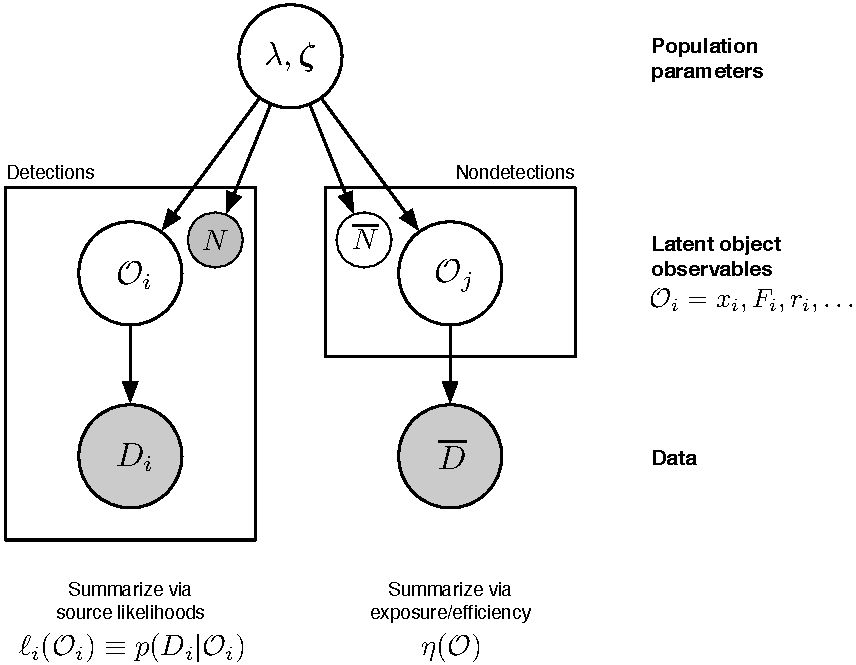
\includegraphics[width=.8\textwidth]{fig/DAG-TLPP}
\end{center}
\caption{Schematic DAG for a thinned latent marked point process model for luminosity function estimation from survey catalog data.
The small $N$ and $\overline{N}$ nodes specify the numbers of replications of the detection and nondetection plates, respectively.}
\label{fig:TLPP}
\end{figure}

Despite these differences with respect to the simpler model structures discussed previously, the structure of the likelihood functions in (\ref{eq:like}) and (\ref{eq:mlike}) is essentially the same as that for conditional density estimation with measurement error (the middle DAG in Fig.~\ref{fig:DAG-TLPP}).
This is because the nondetection part of the DAG in Fig.~\ref{fig:DAG-TLPP} corresponds to a product of exponentials, whose arguments sum in a single integral: the integral on the first line of the likelihood function in (\ref{eq:like}), and in the denominator of the effective densigyt in (\ref{eq:epdf}).
The likelihood or marginal likelihood thus has a single product term, composed of independent factors for each detected object---just the type of structure CUDAHM was designed to sample from.